\chapter{Einleitung}
\label{kap:einleitung}

\section{Zielsetzung}
\label{sec:zielsetzung}

Unter physiologischen Bedingungen liegt die mittlere Lebensdauer der \amid~bei einigen Jahrzehnten bis hin zu mehreren Jahren \cites{Radzicka.}[41]{Berg.2018}. Diese Reaktion kann unter Einfluss von Säuren oder Basen katalysiert werden. Eine weitere Möglichkeit die Hydrolyse der \amid~zu beschleunigen liegt darin, eine äußere Kraft entlang der C-N-Bindungsachse anzulegen. Diese mechanische Aktivierung führt zu einer Beschleunigung der Hydrolyse auf Bruchteile von Sekunden \cites{ClausenSchaumann.2018}. Ziel dieser Arbeit ist daher die Untersuchung der \amid~auf Einzelmolekülebene, indem ein Spacermolekül zwischen die \spitze~eines Rasterkraftmikroskops und einer Substratoberfläche gespannt und die Geschwindigkeitskonstante der Hydrolyse der \amid~unter dem Einfluss einer äußeren Kraft und bei verschiedenen pH-Werten evaluiert wird. Ausgesucht wurden folgende pH-Werte:

\begin{itemize}
	\item 4,5
	\item 7,4
	\item 8
\end{itemize}

Die Untergrenze von pH 4,5 wurde gewählt, sodass noch ausreichen \aminos~auf der \spitze~vorhanden waren, um freie Elektronenpaare für die Kopplungsreaktion der \carboxys~an die \aminos~zur Verfügung zu stellen. Der mittlere pH-Wert von 7,4 stellt die Referenz zu \cites{ClausenSchaumann.2018} dar. Bei der oberen pH-Grenze gilt es darauf zu achten, dass für den experimentellen Zeitrahmen genügend \amid~zwischen Spacermolekül und der \spitze~bzw. der Substratoberfläche gebildet werden können. Die Halbwertszeit der für diese Kopplung essentiellen Verbindungen liegt bei einem pH-Wert von 8,5 nur noch bei wenigen Minuten \cites{Hayworth}.\\
Die Arbeitshypothese lautet dabei wie folgt:

\begin{itemize}
	\item Je basischer das Medium in dem gemessen wurde ist, desto schwieriger ist während der Hydrolysereaktion der Übergang zwischen den Zwischenprodukten (vgl.~Abschnitt~\ref{sec:hydrolyse_der_amidbindung}). Dementsprechend liegt die Geschwindigkeitskonstante der Hydrolyse bei pH 8 in etwa bei der von pH 7,4.
\end{itemize}

Grundgedanke ist, dass die Erhöhung des pH-Wertes die Energiebarriere zwischen den beiden Zwischenprodukten erhöht und damit die Absenkung der Geschwindigkeitskonstante der Amidhydrolyse unter basischer Katalyse kompensiert wird.

\section{Kopplungschemie}
\label{sec:kopplungschemie}

Um eine erfolgreiche Kopplung zwischen den Spacermolekülen und  des Substrats bzw. der \spitze~zu gewährleisten, wurde die gesamte Funktionalisierung auf zwei Schritte aufgeteilt. Zunächst wurde das Substrat bzw. \spitze~mit terminalen Aminogruppen funktionalisiert (s.~Abschnitt~\ref{subsec:oberflächenfunktionalisierung_via_kohlenstoffanker}). Anschließend erfolgte die Aktivierung der Carbonylgruppen am Spacermolekül (vgl.~Abschnitt~\ref{subsec:kopplung_der_spacermoleküle_an_funktionalisierte_oberfläche}). 

\subsection{Oberflächenfunktionalisierung via Kohlenstoffanker}
\label{subsec:oberflächenfunktionalisierung_via_kohlenstoffanker}

Die Oberflächenfunktionalisierung wird schematisch in \abb~\ref{subfig:Hauptreaktion} gezeigt \cite{MichaelF.Pill.2015}. Für die Reaktion ist eine homolytische Spaltung der C-C-Bindungen an der Oberfläche des Substrats der erste Schritt. Anschließend erfolgt die Kopplung von Allylamin ($X~=~NH_2$) an die Substratoberfläche durch die Reaktion mit den entstandenen Radikalen. Mögliche Nebenreaktionen dieser radikalischen Reaktion sind in den \abbn~\ref{subfig:Nebenreaktion-a}~bis~\ref{subfig:Nebenreaktion-c} dargestellt \cite{MichaelF.Pill.2015}.

\begin{figure}[H]
	\begin{subfigure}[h]{\textwidth}
		\centering
		\scalebox{\hscaleOne}{
			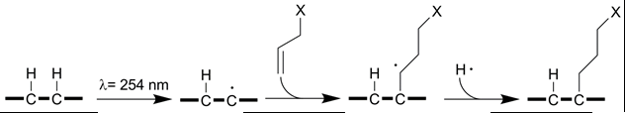
\includegraphics[width=\linewidth]{Abbildungen/OF_Funktionalisierung.png}
		} % scalebox
		\subcaption{}
		\label{subfig:Hauptreaktion}
	\end{subfigure}

	\begin{subfigure}[h]{\textwidth}
		\centering
		\scalebox{\hscaleOne}{
			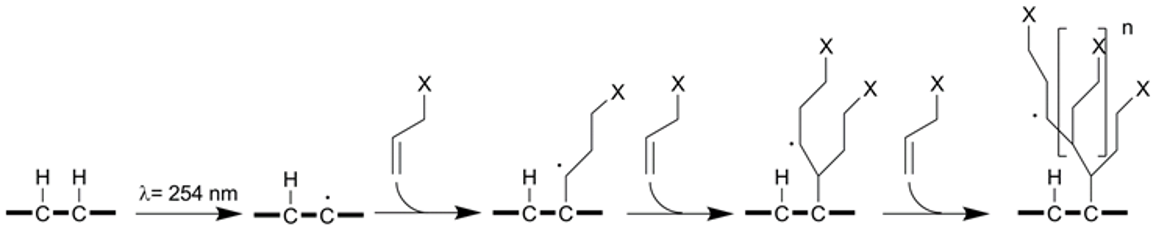
\includegraphics[width=\linewidth]{Abbildungen/OF_Funktionalisierung_Nebenreaktionen_a.png}
		} % scalebox
		\subcaption{}
		\label{subfig:Nebenreaktion-a}
	\end{subfigure}

	\begin{subfigure}[h]{\textwidth}
		\centering
		\scalebox{\hscaleOne}{
			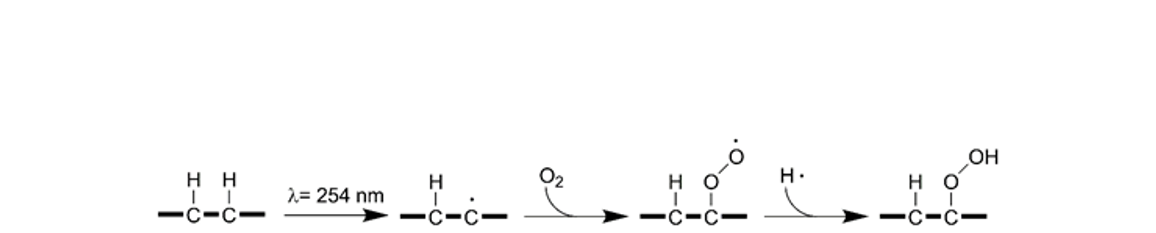
\includegraphics[width=\linewidth]{Abbildungen/OF_Funktionalisierung_Nebenreaktionen_b.png}
		} % scalebox
		\subcaption{}
		\label{subfig:Nebenreaktion-b}
	\end{subfigure}

	\begin{subfigure}[h]{\textwidth}
		\centering
		\scalebox{\hscaleOne}{
			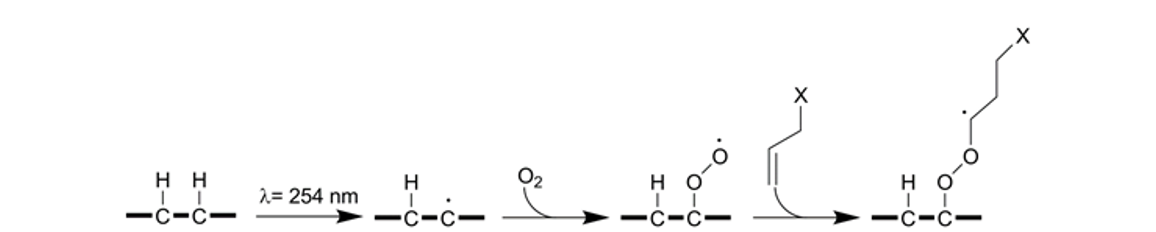
\includegraphics[width=\linewidth]{Abbildungen/OF_Funktionalisierung_Nebenreaktionen_c.png}
		} % scalebox
		\subcaption{}
		\label{subfig:Nebenreaktion-c}
	\end{subfigure}
	
	\caption{Reaktion der Oberflächenfunktionalisierung. a) Start der radikalischen Reaktion ist die Bestrahlung der Kohlenstoffoberfläche des Substrats und der \spitze~durch UV-Licht der Wellenlänge $\lambda~=~254~nm$. Im Verlauf der Reaktion wird ein Allylamin-Molekül ($X~=~NH_2$) an die Oberflächen von \spitze~und Substrat angelagert. Das ungepaarte Elektron am Kohlenstoffrückgrat des Allylamin wird über ein Wasserstoffradikal abgesättigt. Während der Funktionalisierung sind folgende Nebenreaktionen möglich: b). Baumartiges Wachstum von Allylamin-Molekülen, bedingt durch eine zu hohe Allyaminkonzentration. b) Terminierung des Substrats/ \spitze~mit \carboxys~durch den Einbau von molekularem Sauerstoff. c) Bildung von Peroxid artigen Strukturen zwischen Substrat/ \spitze~und Allylamin, bedingt durch den Einbau von molekularem Sauerstoff.}
	
	\label{fig:OF_Funktionalisierung}
\end{figure}

\subsection{Kopplung der Spacermoleküle an funktionalisierte Oberflächen}
\label{subsec:kopplung_der_spacermoleküle_an_funktionalisierte_oberfläche}

Die Bildung der \amid~erfolgt durch eine  Standard Kopplungschemie über \ac{EDC} und \ac{NHS} \cite{Hermanson.2013,MichaelF.Pill.2015}. Als Spacermolekül wurde \ac{CMA} verwendet. \abb~\ref{fig:Kopplungschemie} zeigt die Kopplung von \spacer~und Substrat bzw. \spitze. $R_1$ stellt den \spacer~dar, dessen \carboxys~zunächst durch \ac{EDC} aktiviert und anschließend durch \ac{NHS} in \ester~überführt werden. Die Bildung der \amid~erfolgt schließlich zwischen den \estern~und den \aminos~des funktionalisierten Substrats bzw. \spitze~($R_2$). Wie aus \abb~ \ref{fig:Kopplungschemie} zu erkennen ist, wird \ac{NHS} durch die Reaktion mit einem primären Amin im Kreislauf gehalten. \ac{EDC} hingegen reagiert während der Aktivierung der \carboxys~zu einem nicht reaktiven Isourea ab.

\begin{figure}[H]
	\begin{flushleft}
		\scalebox{\hscaleOne}{\begin{minipage}{\textwidth}
				\schemedebug{false}
				\schemestart
				\chemname{\Rest}{Carbonsäure} 
				\arrow(.south--.north west){-U>[*{0.south west}\chemname{\EDC}{EDC}][][][.5][]}[-90,4] 
				\chemname{\OAcylisourea}{O-Acylisourea Zwischenprodukt}
				\arrow{-U>[*{0.south}\chemname{\NHS}{NHS}][][][.5][]}[,3]
				\chemname{\Ester}{NHS Ester Zwischenprodukt}
				\arrow{-U>[*{0.north east}\chemname{\PrimAmin}{Primäres Amin}][*{0.east}\chemname{\NHS}{NHS}][][.3][60]}[90,4]
				\chemname{\Amidbindung}{Bildung der Amidbindung}
				\schemestop
			\end{minipage}
		}
	\end{flushleft}
	\caption[Reaktionsschema der Kopplungschemie über \acs*{EDC} und \acs*{NHS}]{Reaktionsschema der Kopplungschemie über \acs*{EDC} und \acs*{NHS}: Beginn der Kopplung ist die Aktivierung eines Moleküls mit Carboxylgruppe ($R_1-COOH$) mittels \acs*{EDC}. Das dabei entstandene Isourea Zwischenprodukt wird in einem zweiten Schritt über Zufuhr von \acs*{NHS} das aktivierte \ester~Zwischenprodukt gebildet. Zuletzt wird über den Angriff eines Nucleophils ($R_2-NH_2$) die Amidbindung gebildet.}
	\label{fig:Kopplungschemie}
\end{figure}

\section{Hydrolyse der Amidbindung}
\label{sec:hydrolyse_der_amidbindung}

Die Hydrolyse ist eine spezielle Art der Solvolyse, die Auflösung einer chemischen Bindung unter Beteiligung von Lösungsmittelmolekülen. Sie verläuft nach dem $S_N2$-Mechanismus pseudo-erster Ordnung, da die Konzentration des Lösungsmittel annähernd konstant bliebt \cite[91]{Hadener.2006}. Alternativ kann die Hydrolyse der \amid~auch als eine Reaktionskaskade einer Additionsreaktion, gefolgt von einer Eliminierungsreaktion angesehen werden \cite[288]{Latscha.2016}. Unter neutralen Bedingungen verläuft die Amidhydrolyse nach dem Schema, dargestellt in \abb~\ref{fig:amid_neutral} ab \cites[288]{Latscha.2016}{Zahn.2004b}.\\

Zunächst bindet ein Wassermolekül mit einem freien Elektronenpaar am Carbonylkohlenstoff von N1. Dabei dissoziiert das addierte Wasser und ein Proton wird direkt, über einen Grotthuß-artigen Mechanismus auf den Stickstoff des \ac{TZP} N2 übertragen. Anschließend lagern sich die Elektronen in N2 um und regenerieren im zweiten Schritt die \carboxys~am \spacer~($R_1-COOH$) N3 und die \amino~auf dem Substrat bzw. der \spitze~($R_2-NH_2$) N4.

\begin{figure}[H]
	\begin{flushleft}
		\scalebox{\hsclaeChemfig}{\begin{minipage}{\textwidth}
				\setchemfig{scheme debug = false}
				\schemestart
				\Wasser
				\hspace{1cm}
				\chemname{\Amidbindung}{N1}
				\chemmove[shorten <= 5pt, shorten >= 2pt]{\draw[dashed](n1)..controls +(north east:1.5cm) and +(south:2.75cm)..(n2);}
				\arrow{<=>}
				\chemname{\AmidbindungII}{N2}
				\chemmove[shorten <= 5pt, shorten >= 2pt]{\draw[dashed](n4)..controls +(east:0.5cm) and +(east:0.75cm)..(n3);
					\draw[dashed](n5)..controls +(north east:0.5cm) and +(north:0.5cm)..(n6);}
				\arrow{<=>}
				\chemname{\Acid}{N3} \+ \chemname{\PrimAmin}{N4}
				\schemestop
			\end{minipage}
		}
	\end{flushleft}
	\caption[Hydrolyse der Amidbindung im neutralen Milieu]{Hydrolyse der Amidbindung im neutralen Milieu. Der Angriff des Wassers erfolgt am Carbonylkohlenstoff von N1. Dabei dissoziiert das Wassermolekül und ein Proton wird über einen Grotthuß artigen Mechanismus auf das Stickstoffatom von N2 übertragen. Nach einer Reihe interner Elektronenumlagerungen bricht im zweiten Schritt die Amidbindung unter Rückbildung der \spacer~($R_1-COOH$) N3 und des Substrats ($R_2-NH_2$) N4.}
	
	\label{fig:amid_neutral}
\end{figure}

\subsection{Sauer katalysierte Amidhydrolyse}
\label{subsec:sauer_katalysierte_amidhydrolyse}

Die saure Katalyse der Amidhydrolyse beruht auf der erhöhten Polarität der \carboxy~durch Addition eines Protons an das Carbonylsauerstoff. Die Reaktion läuft dabei nach dem Schema, dargestellt in \abb~\ref{fig:amid_sauer} ab \cites[288]{Latscha.2016}{Zahn.2004b}{Zahn.2003}\\

Nach der Bildung des Carbeniumions (S1) erfolgt der nucleophile Angriff des Wassers. Dieses dissoziiert dabei in ein \ch{OH-}-Ion und ein \ch{H+}-Ion. Während das \ch{OH-}-Ion an den positiv geladenen Carbonylkohlenstoff addiert wird, geht das gebildete \ch{H+}-Ion in Lösung. Im zweiten Schritt wird das \ac{TZP} (S2) durch ein weiteres \ch{H+}-Ion aus der Lösung am Stickstoffatom protoniert und S3 gebildet. Im letzten Schritt wird die \amid~durch eine Reihe interner Elektronenumlagerungen gebrochen. Dabei werden die \carboxys~des \spacer~($R_1-COOH$) S4 und \aminos~des Substrats bzw. der \spitze~($R_2-NH_3^+$) S5 regeneriert.\\

Die Reaktionsmechanismen der Amidhydrolyse im Sauren, sowie im Neutralen sind sich sehr ähnlich. Der Unterschied besteht in der Art und Weise wie das Stickstoffatom protoniert wird, dies zeigt eine theoretische Studie von D.~Zahn~\textit{et al}.~\cites{Zahn.2004b}.

\begin{figure}[H]
	\begin{flushleft}
		\scalebox{\hsclaeChemfig}{\begin{minipage}{\textwidth}
				\setchemfig{scheme debug = false}
				\schemestart
				\Wasser
				\hspace{0.1cm}
				\chemname{\AmidbindungIII}{S1}
				\chemmove[shorten <= 5pt, shorten >= 5pt]{\draw[dashed](n1)..controls +(north east:1.5cm) and +(240:2.75cm)..(pa1);}
				\arrow{<=>[-H$_{\mathrm{aq}}^{\tiny +}$][+H$_{\mathrm{aq}}^{\tiny +}$]}
				\chemname{\AmidbindungIV}{S2}
				\arrow{<=>[+H$_{\mathrm{aq}}^{\tiny +}$][-H$_{\mathrm{aq}}^{\tiny +}$]}
				\chemname{\AmidbindungV}{S3}
				\chemmove[shorten <= 2pt, shorten >= 2pt]{\draw[dashed](av2)..controls +(north:1.5cm) and +(west:1.5cm)..(av1);
					\draw[dashed](av4)..controls +(350:0.75cm) and +(south east:0.75cm)..(av3);}
				\arrow{<=>}
				\chemname{\Acid}{S4} \+ \chemname{\PrimAminII}{S5}
				\schemestop
			\end{minipage}
		}
	\end{flushleft}
	\caption[Reaktionsmechanismus der sauer katalysierten Amidhydrolyse]{Reaktionsmechanismus der sauer katalysierten Amidhydrolyse. Das durch die Protonierung des Carbonylsauerstoff entstandene Carbeniumion S1 ist sehr viel reaktiver als die unveränderte Carbonylgruppe. Der nucleophile Angriff kann daher sehr viel schneller erfolgen als vor der Protonierung. Während des nucleophilen Angriffs dissoziiert das Wassermolekül, das gebildete \ch{H+}-Ion geht in Lösung, das \ch{OH-}-Ion wird an das Carbonylkohlenstoff addiert und bildet das tetraedrische Zwischenprodukt S2. In einem dritten Schritt wird durch ein weiteres \ch{H+}-Ion das Stickstoffatom protoniert, wodurch das Zwischenprodukt S3 gebildet wird. Nach einer Reihe interner Elektronenumlagerungen bricht die Amidbindung unter Rückbildung des \spacers~($R_1-COOH$) S4 und des Substrat/ \spitze~($R_2-NH_3^+$) S5.}
	
	\label{fig:amid_sauer}
\end{figure}

\subsection{Basisch katalysierte Amidhydrolyse}
\label{subsec:basisch_katalysierte_amidhydrolyse}

Während der basischen Katalyse der Amidhydrolyse wird in einer vorgelagerten Gleichgewichtsreaktion aus dem weniger nucleophilen Wasser das sehr viel nucleophilere \ch{OH-}-Ion gebildet. Danach läuft die Reaktion nach dem Schema in \abb~\ref{fig:amid_basisch} ab \cites[288]{Latscha.2016}{Zahn.2004b}{Zahn.2004}\\

Das gebildete \ch{OH-}-Ion greift den Carbonylkohlenstoff der Amidbindung B1 an und es wird das \ac{TZP} B2 gebildet. Nachdem ein solvatisiertes \ch{H+}-Ion aus der Lösung in die Nähe von B2 diffundiert ist, wird das Stickstoffatom in B2 protoniert und es bildet sich das \ac{ZI} B3. Anschließend erfolgt nach einer Reihe interner Elektronenumlagerungen im letzten Schritt der Bruch der Amidbindung und es wird die \carboxy~am \spacer~($R_2-COOH$, B4), sowie die \amino~auf dem Substrat regeneriert.\\

Mit steigendem pH-Wert ist es außerdem möglich, dass die verbleibenden \carboxy~am \ac{ZI} (B3) zusätzlich deprotoniert wird \cites{Zahn.2004}. Dadurch entsteht statt der Carbonsäure in B4 das Carboxylation.

\begin{figure}[H]
	\begin{flushleft}
		\scalebox{\hsclaeChemfig}{\begin{minipage}{\textwidth}
			\setchemfig{scheme debug = false}
			\schemestart
				\OHIon
				\hspace{0.5cm}
				\chemname{\Amidbindung}{B1}
				\chemmove[shorten <= 5pt, shorten >= 2pt]{\draw[dashed](oh)..controls +(330: 1cm) and +(260:1cm)..(n2);
				}
				\arrow{<=>}
				\chemname{\AmidbindungVI}{B2}
				\arrow{<=>[+H$_{\mathrm{aq}}^{\tiny +}$][-H$_{\mathrm{aq}}^{\tiny +}$]}
				\chemname{\AmidbindungVII}{B3}
				\chemmove[shorten <= 5pt, shorten >= 2pt]{\draw[dashed](aoh2)..controls +(east:0.5cm) and +(east:0.75cm)..(aoh1);
					\draw[dashed](aoh3)..controls +(north east:0.5cm) and +(north:0.5cm)..(aoh4);
				}
				\arrow{<=>}
				\chemname{\Acid}{B4} \+ \chemname{\PrimAmin}{B5}
			\schemestop
		\end{minipage}
	}
	\end{flushleft}
	\caption[Reaktionsmechanismus der basisch katalysierten Amidhydrolyse]{Reaktionsmechanismus der basisch katalysierten Amidhydrolyse. Durch eine vorgelagerte Gleichgewichtsreaktion entsteht aus Wasser ein nucleophileres \ch{OH-}-Ion. Dieses greift statt Wasser am Carbonylkohlenstoff der Amidbindung von B1 an und bildet das tetraedrische Zwischenprodukt B2. Im zweiten Schritt diffundiert ein \ch{H+}-Ion aus der Lösung und protoniert das Stickstoffatom in B2. Dabei wird das zwitterionische Zwischenprodukt B3 gebildet. Nach einer Reihe interner Elektronenumlagerungen bricht die Amidbindung unter Rückbildung des \spacers~($R_1-COOH$) B4 und des \substrats/ \spitze~($R_2-NH_2$) B5.}
	
	\label{fig:amid_basisch}
\end{figure}

\subsection{Energieprofil der Amidhydrolyse ohne Krafteinfluss}
\label{subsec:energieprofil_der_amidhydrolyse_ohne_krafteinfluss}
Energetisch gesehen durchläuft die Hydrolyse der \amid~zwei prominenten Barrieren, wie in \abb~\ref{fig:energieprofil_ohne_kraft} dargestellt \cite{Zahn.2003,Zahn.2004,Zahn.2004b}. Um den \ac{UZ}1 - die innere Barriere - zu überwinden wird eine Aktivierungsenergie von ca. $147~kJ~mol^{-1}$ im neutralen Milieu~\cites{Zahn.2004b}, $78~kJ~mol^{-1}$ im sauren Milieu~\cites{Zahn.2003} und ca. $66~kJ~mol^{-1}$ im basischen Milieu~\cites{Zahn.2004} benötigt. Für den \ac{UZ}2 - die äußere Barriere - weitere $38~kJ~mol^{-1}$ im sauren Milieu~\cites{Zahn.2003} und $72~kJ~mol^{-1}$ im basischen Milieu\cites{Zahn.2004}. Es sind keine Angaben für \ac{UZ}2 im neutralen Milieu verfügbar. Der Übergang von \ac{TZP} zum \ac{ZI} wird als barrierefrei angesehen. Für die Rückreaktion des \ac{TZP} zum Eduktzustand im sauren/ basischen Milieu ist lediglich eine Aktivierungsenergie von $12-20~kJ~mol^{-1}$ notwendig~\cite{Zahn.2004,Zahn.2003}. Aufgrund dieser Tatsache ist die Rückreaktion vom \ac{TZP} bzw. \ac{ZI} zum Eduktzustand wahrscheinlicher, als die Vorwärtsreaktion zum Produktzustand und erklärt die lange Lebensdauer der \amid~von mehreren Dekaden bis hin zu mehreren Jahrhunderten \cite{Radzicka.,Berg.2018}.

\begin{figure}[h]
	\centering
	\scalebox{\hscaleOne}{
		\includegraphics[width=\linewidth]{Abbildungen/Energieprofil_ohne_Kraft.png}
	} % scalebox
	\caption[Energieprofil der Amidhydrolyse ohne Einfluss einer äußeren Kraft]{Energieprofil der Amidhydrolyse ohne Einfluss einer äußeren Kraft. Die Höhe der inneren Barriere \acs*{UZ}1 liegt bei $147~kJ~mol^-1$~\cite{Zahn.2004b} (neutral), $78~kJ~mol^{-1}$\cite{Zahn.2003} (sauer katalysiert) und $66~kJ~mol^{-1}$~\cite{Zahn.2004} (basisch katalysiert). Die Höhe der äußeren Barriere \acs*{UZ}2 liegt bei $38~kJ~mol^{-1}$~\cite{Zahn.2003} (sauer katalysiert) und $72~kJ~mol^{-1}$~\cite{Zahn.2004} (basisch katalysiert). Für den Bruch der Amidbindung im neutralen Milieu liegen keine Daten vor. Die Überführung des \acs*{TZP} in \acs*{ZI} läuft annähernd barrierefrei.}
	\label{fig:energieprofil_ohne_kraft}
\end{figure}

\subsection{Bindungskinetik unter Krafteinfluss}
\label{subsec:bindungskinetik_unter_krafteinfluss}

Ein bekanntes Modell, um die Kraftabhängigkeit chemischer Bindungen zu beschreiben, stammt von Zhurkov und Bell \cite{Zhurkov.1984,Bell.1978}:

\begin{equation}
	E_a(F)~=~\Delta E_{a,0}~-~F \cdot \Delta x^\ddag
	\label{eq:bell_modell}
\end{equation}

Dabei steht $\Delta E_{a,0}$ für die Aktivierungsenergie des Bindungsbruchs ohne Krafteinfluss (hier die Höhe von \ac{UZ}2), $\Delta x^{ddag}$ für den Abstand von einem Produktzustand zu einem Übergangszustand entlang der Reaktionskoordinate (hier von \ac{ZI} zu \ac{UZ}2).\\

In \abb~\ref{fig:energieprofil_mit_kraft} sind exemplarisch die Energieprofile der basisch katalysierten Amidhydrolyse bei verschiedenen Kräften, berechnet nach dem Modell von Zhurkov und Bell, dargestellt. Ab einer Kraft von $500~pN$ (\abb~\ref{fig:energieprofil_mit_kraft}, blauer Graph) liegen \ac{UZ}1 und \ac{UZ}2 in etwa bei derselben Aktivierungsenergie ($64~kJ~mol^{-1}$ bzw. $68~kJ~mol^{-1}$) und \ac{UZ}1 beginnt die Kinetik der Reaktion zu bestimmen. Bei einer Kraft von $800~pN$ (\abb~\ref{fig:energieprofil_mit_kraft}, roter Graph) liegt \ac{UZ}2 ($49~kJ~mol^{-1}$) deutlich unterhalb von \ac{UZ}1 ($63~kJ~mol^{-1}$) und \ac{UZ}1 dominiert die Kinetik der Reaktion vollständig.\\

% Energieprofil mit Kraft
\begin{figure}[h]
	\centering
	\scalebox{\hscaleOne}{
		\includegraphics[width=\linewidth]{Abbildungen/Energieprofil_mit_Kraft.png}
	} % scalebox
	\caption[Energieprofil der Amidhydrolyse unter dem Einfluss einer äußeren Kraft]{Energieprofil der Amidhydrolyse unter dem Einfluss einer äußeren Kraft am Beispiel der basisch katalysierten Hydrolyse. Die Energien einzelner \acs*{UZ} und \acs*{ZI} wurden über das Modell von Zhurkov und Bell berechnet. Für eine Zugkraft von 500 pN (blau) rückt \acs*{UZ}2 (ca. $68~kJ~mol^{-1}$) in den Bereich von \acs*{UZ}1 (ca. $64~kJ~mol^{-1}$). Bei einer Zugkraft von 800 pN (rot) liegt \acs*{UZ}2 (ca. $49~kJ~mol^{-1}$) unterhalb von \acs*{UZ}1 (ca. $49~kJ~mol^{-1}$).}
	\label{fig:energieprofil_mit_kraft}
\end{figure}


Zusammen mit \gl~\ref{eq:bell_modell} und der Arrhenius-Gleichung erhält man die kraftabhängige Geschwindigkeitskonstante $k(F)$ für den Bruch einer chemischen Bindung\footnote{Unter Krafteinwirkung entlang der Bindungsachse} \cite{RibasArino.2012}:

\begin{equation}
	k(F)~=~k_0 \cdot e^{\frac{F \cdot \Delta x^\ddag}{k_B T}}
	\label{eq:k_kraftabhängig}
\end{equation}

Mit $k_B$ der Boltzmannkonstante, $k_0$ der Geschwindigkeitskonstante des Bindungsbruchs ohne äußere Kraft und $T$ der absoluten Temperatur in Kelvin. Der allgemeine Zusammenhang zwischen Geschwindigkeitskonstante und der Zeitkonstante eines Prozesses lautet:

\[ k~=~\frac{1}{\tau} \]

Damit ergibt sich der Ausdruck für die Kraftabhängige, mittlere Lebensdauer \cite{Glockner.2011}:

\begin{equation}
	\tau(F)~=~\tau_0 \cdot e^{- \frac{F \cdot \Delta x^\ddag}{k_BT}}
	\label{eq:tau_kraftabhängig}
\end{equation}

Wobei $\tau_0$ die mittlere Lebensdauer einer chemischen Bindung ohne äußre Kraft bezeichnet. Wird eine Kraft entlang der C-N-Bindung eines Amids angelegt, so wird die äußere Barriere effektiver abgesenkt, als die innere Barriere \cite{Xia.2011,Tian.2013}. Dieses Verhalten wird damit begründet, dass die Reaktionskoordinate für die innere Barriere\footnote{Meist der Abstand zwischen dem Sauerstoffatom eines angreifenden \ch{H20}-Moleküls bzw. \ch{OH-}-Ions und dem Carbonylkohlenstoff.} nahezu senkrecht zur Kraftrichtung läuft. Die Reaktionskoordinate für die äußere Barriere\footnote{Meist der Abstand des Carbonylkohlenstoff und dem Stickstoffatom des Amids.} hingegen liegt parallel zur äußeren Kraft. Die beiden Reaktionskoordinaten sind voneinander unabhängig. Auf Force-Clamp-Experimente übertragen bedeutet das, dass die Änderung des C-N-Abstandes nicht die Geschwindigkeit beeinflusst, mit der ein Nucleophil die Carbonylgruppe angreift (vgl.~Abschnitt~\ref{sec:hydrolyse_der_amidbindung}).\\

In dieser Arbeit ist die Zeit, bei der eine spezifische Bindung bricht, der experimentell zugängliche Parameter. Sinnvoll ist daher die quantitative Bestimmung von $k$ durch die Betrachtung des Reaktion von  \ac{ZI} zum Produktzustand als eine Reaktion 1. Ordnung \cite{MichaelF.Pill.2015}:

\begin{equation}
	N(t)~=~N_0 \cdot e^{-k \cdot t}
	\label{eq:exponentieller_zerfall}
\end{equation}

$N(t)$ steht für die Anzahl der zum Zeitpunkt $t$ intakten \amide~und $N_0$ für die Anzahl aller gemessenen \amide. Durch den Fit dieses exponentiellen Zerfalls an die Messdaten kann $k$ als freier Parameter bestimmt werden.\\
In manchen Fällen kommt es vor, dass in den gemessenen Daten zwei Zerfallsprozesse auftreten. Für solche Fälle lässt \gl~\ref{eq:exponentieller_zerfall} zu einem biexponentiellen Zerfall erweitern:

\begin{equation}
	N(t)~=~N_0 \cdot [A \cdot e^{-k_1 \cdot t}~+~(A~-~1) \cdot e^{-k_2 \cdot t}]
	\label{eq:biexponentieller_zerfall}
\end{equation}

Hierbei stehen die beiden Geschwindigkeitskonstanten $k_1$ und $k_2$ für einen schnellen, bzw. für einen langsamen Prozess. Der Mischungskoeffizient $A$ ist definiert als:

\[ A~=~\frac{N_{0,1}}{N_0} \]

Und

\[ (1~-~A)~=\frac{N_0~-~N_{0,1}}{N_0}~=~\frac{N_{0,2}}{N_0} \]

Wobei $N_{0,1}$ für die Anzahl aller Spezies mit $k_1$ bzw. $N_{0,2}$ für die Anzahl aller Spezies mit $k_2$ und $N_0~=~N_{0,1}~+~N_{0,2}$ für die Anzahl aller gemessen Bindungen.

\section{Rasterkraftmikroskop}
\label{sec:rasterkraftmikroskop}

Das Rasterkraftmikroskop (\ac{AFM}) wurde ursprünglich von Binnig, Quate und Gerber im Jahr 1986 entwickelt \cite{Binnig.1986}. Es diente als Weiterentwicklung des Rastertunnelmikroskops zur Abbildung von Oberflächen nichtleitender Proben. Den heutigen Aufbau des \acp{AFM} und eine Übersicht über einige Anwendungen gibt z.B. McConney \textit{et al}. \cite{McConney.2010}. Eine schematische Darstellung des \acp{AFM} zeigt \abb~\ref{fig:afm_schema}. Das Herzstück des \acp{AFM} ist eine \spitze~am Ende eines Cantilevers, auf dessen Rückseite ein Laserstrahl ausgerichtet wird (\abb~\ref{fig:afm_schema}a). Die Reflektion des Laserstrahls wird von einer segmentierten Photodiode erfasst (\abb~\ref{fig:afm_schema}b). Wird die Oberfläche mit der sehr feinen Messspitze\footnote{Im Idealfall sitzt ein einzelnes Atom am Ende der Spitze.}  (\abb~\ref{fig:afm_schema}c)) über die x-, y- und z- Piezos (\abb~\ref{fig:afm_schema}d)) abgerastert, führen Wechselwirkungen von \spitze~und Substrat zu einer Auslenkung des Cantilevers. Diese Auslenkung wird durch die segmentierte Photodiode gemessen.\\

\begin{figure}[h]
	\centering
	\scalebox{\hscaleOne}{
		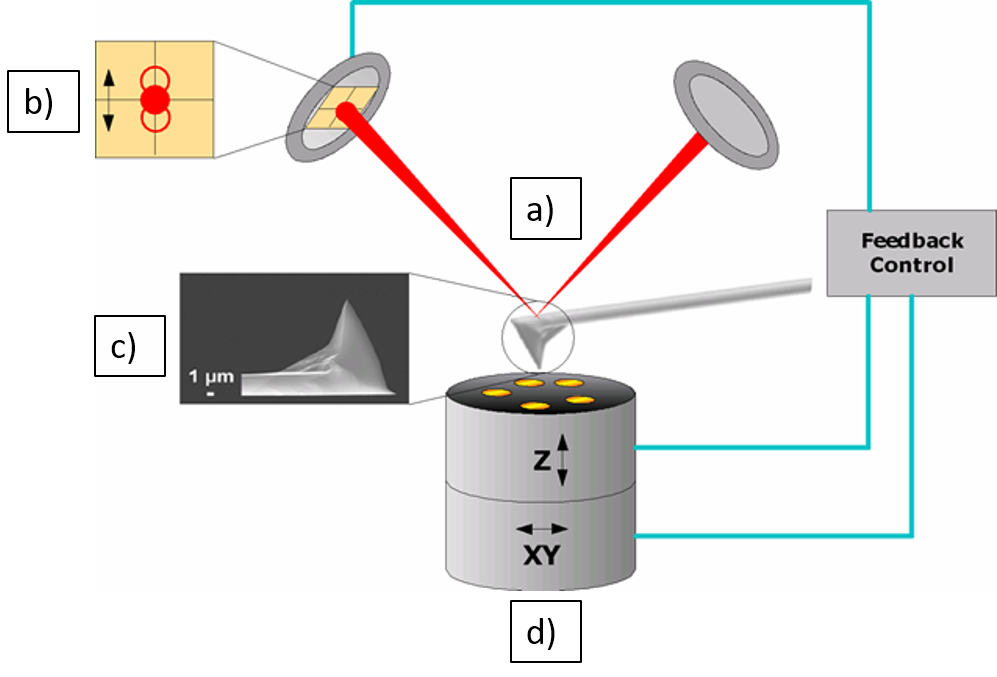
\includegraphics[width=\linewidth]{Abbildungen/AFM.png}
	} % scalebox
	\caption[Schematische Darstellung des Rasterkraftmikroskops]{Schematische Darstellung des Rasterkraftmikroskops. Die wichtigsten Komponenten sind: a) Cantilever mit ausgerichtetem Laserstrahl. b) Segmentierte Photodiode. c) Die Messspitze am Ende des Cantilever. d) x-, y- und z-Piezos.}
	\label{fig:afm_schema}
\end{figure}

Für die durchgeführten einzelmolekülspektroskopischen Untersuchungen (\ac{SMFS}), wird zwischen \spitze~und Substrat, mittels der in Abschnitt~\ref{subsec:kopplung_der_spacermoleküle_an_funktionalisierte_oberfläche} beschriebenen Chemie, ein \spacer~gebunden. Beim Zurückziehen des z-Piezos wird das Molekül gestreckt und der Cantilever ausgelenkt.\\

\ac{SMFS}-Experimente werden anhand der Kraftdynamik am \space~ charakterisiert. Wird die wirkende Kraft zeitlich konstant gehalten, wird von Force-Clamp-\ac{SMFS} gesprochen.\\
In Force-Clamp-Experimenten wird der \spacer~bis zu einer Kraft gestreckt, bei der noch kein Bindungsbruch stattfindet. Dabei wird die Zeit gemessen, bis die Bindung durch thermisch aktivierte Prozesse bricht.\\

Wirkt die Kraft am \spacer~zeitlich nicht konstant, wird von Force-Ramp-Experimenten gesprochen.\\
In Force-Ramp-Experimenten wird das Spacermolekül mit konstanter Geschwindigkeit in z-Richtung gestreckt. Der z-Piezo wird dabei bis zum Bindungsbruch des \spacer~an den Kopplungspunkten (\spitze~oder Substrat) zurückgezogen.

\section{Einzelmolekülspektroskopie am Rasterkraftmikroskop}
\label{sec:einzelmolekülspektroskopie_am_rasterkraftmikroskop}

\subsection{Molekularer Aufbau des Versuchssystems}
\label{subsec:molekularer_aufbau_des_Versuchssystems}

Der Fokus dieser Arbeit liegt auf der Untersuchung der \amid~ (Rot dargestellte Atomgruppe in \abb~\ref{fig:molekularer_aufbau}). Durch die verwendete Kopplungschemie (vgl. Reaktionsschema aus \abb~\ref{fig:Kopplungschemie}) bildet sich die \amid~zwischen den primären \aminos~von Substrat bzw. \spitze~und den \carboxys~von \ac{CMA}. Die Anzahl an \ac{CMA}-Monomeren zischen den \amide~ist beliebig. Der vollständige molekulare Aufbau des Versuchssystems, wie in \abb~\ref{fig:molekularer_aufbau} dargestellt, zeigt exemplarisch die Verbindung von Substrat und \spitze.

\begin{figure}[h]
	\centering
	\scalebox{\hscaleZero}{
		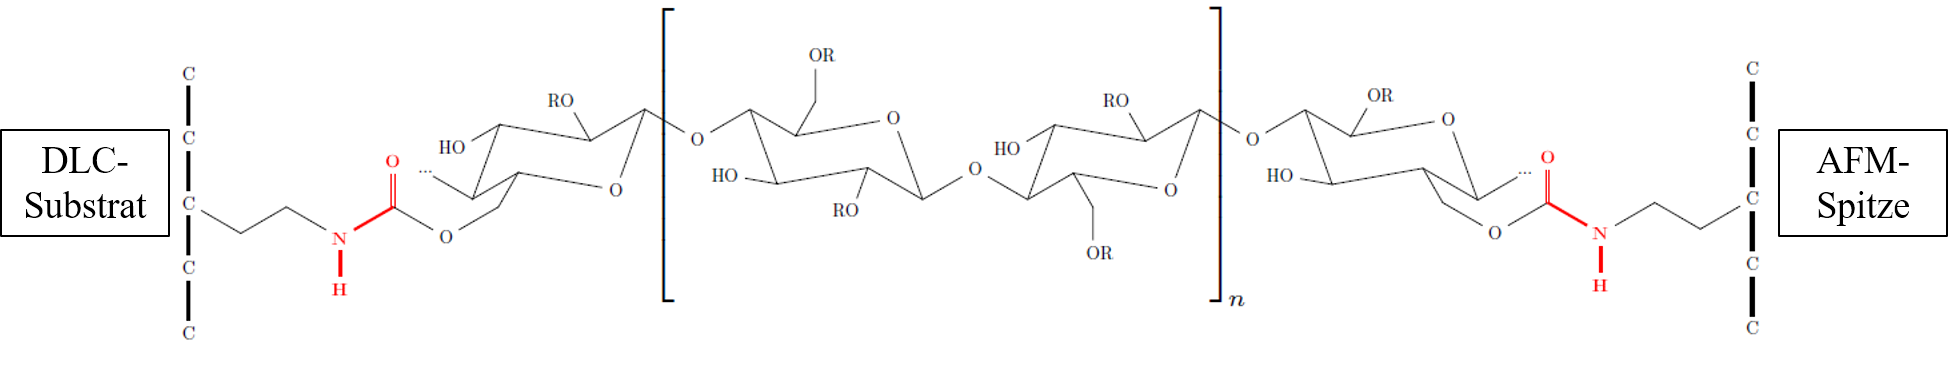
\includegraphics[width=\linewidth]{Abbildungen/molekularer_aufbau.png}
	} % scalebox
	\caption[Molekularer Aufbau der \acs*{SMFS}-Experimente]{Molekularer Aufbau der \acs*{SMFS}-Experimente. In rot sind die untersuchten Amidbindungen zwischen Allylamin und \acs*{CMA} dargestellt.}
	\label{fig:molekularer_aufbau}
\end{figure}

\subsection{Kraftkurven}
\label{subsec:kraftkurven}

In \ac{SMFS}-Experimenten kann die Kraft als Funktion des Wegs (Kraft-Abstand-Kurven), oder als Funktion der Zeit (Kraft-Zeit-Kurven) dargestellt werden. In der Kraft-Abstand-Darstellung lassen sich \ac{CMA}-Spezifische Einzelmolekülinteraktionen identifizieren und in der Kraft-Zeit-Darstellung lässt sich die Clampzeit ermitteln. Um kleinere Abrisse oder Sprünge in der Kraft besser zu erkennen, bietet sich die Weg-Zeit Darstellung der Kraftkurven an. Anhand dieser Darstellungsart lässt sich aus dem Graphen die Geschwindigkeit des z-Piezos ermitteln. Die Steigung ist im Betrag umso größer, je höher die Geschwindigkeit des Piezos war. Bei Abrissen steht der Graph annähernd senkrecht zur Zeit-Achse. \\

Es wurden an einer Probe Force-Ramp-, sowie Force-Clamp-Experimente durchgeführt. Letztere dienen ausschließlich des Zwecks zu überprüfen, ob \ac{CMA}-Spezifische Einzelmolekülinteraktionen auftraten. Force-Clamp-Experimente hingegen werden genutzt, um Abrisszeiten und somit die Geschwindigkeitskonstante der Experimente zu bestimmen.\\

Eine typische Kraftkurve der Force-Ramp-Experimente zeigt \abb~\ref{fig:force_ramp_kurve}. Diese Kurven sind insgesamt in drei Segmente untergliedert:

\begin{enumerate}
	\renewcommand\labelenumi{\bfseries\theenumi.}
	
	\item Hinfahrkurve (\abb~\ref{fig:force_ramp_kurve}, blau)
	\item Ruhezeit (\abb~\ref{fig:force_ramp_kurve}, Orange)
	\item Rückfahrkurve (\abb~\ref{fig:force_ramp_kurve}, Gelb)
	
\end{enumerate}

Im 1. Segment wird die \spitze~mit einer bestimmten Geschwindigkeit (hier $6~µm~s^{-1}$) an das Substrat angenähert, bis eine vorgegebene Auslenkung des Cantilevers (hier $250~pN$) erreicht ist. Um der Ausbildung von \amid~genügend Zeit zu geben, ruht die \spitze~im 2. Segment für ca. 3 Sekunden bei konstanter Kraft auf dem Substrat. Im 3. Segment wird die \spitze~mit einer bestimmten Geschwindigkeit (hier $6~µm~s^{-1}$) wieder von der Substratoberfläche entfernt. Dabei wird der \spacer~bis zum Bruch der \amid~zwischen \spacer~und Substrat bzw. \spitze~gestreckt. Eine vollständige Zusammenstellung der Parameter für ein Force-Clamp-Experiment enthält Tabelle~\ref{tab:force-ramp-parameter} in Abschnitt~\ref{subsec:durchführung_von_clamp/_ramp_versuchen}.\\

\begin{figure}[h]
	\centering
	\scalebox{\hscaleZero}{
		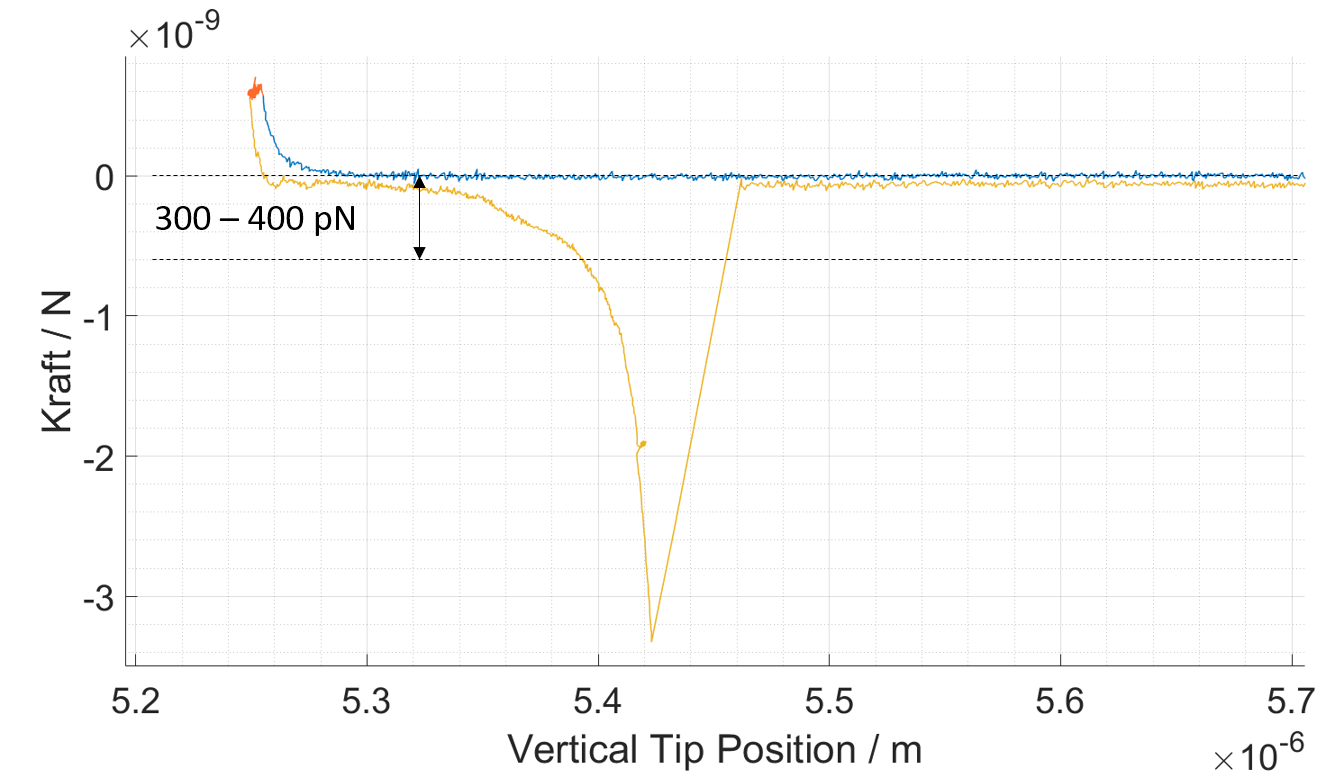
\includegraphics[width=\linewidth]{Abbildungen/Bsp_Force_Ramp_III.png}
	} % scalebox
	\caption[Beispiel einer Force-Ramp-Kraftkurve]{Beispiel einer Force-Ramp-Kraftkurve (Kraft-Abstand-Kurve). Blau: Hinfahrkurve. Orange: Ruhezeit. Gelb: Wegfahrkurve. Hervorgehoben ist das \acs*{CMA}-Spezifische Plateau bei 300 - 400 pN.}
	\label{fig:force_ramp_kurve}
\end{figure}

Typische Ergebnisse aus Force-Clamp-Experimenten zeigt \abb~\ref{fig:force_clamp_kurve}. Dabei zeigt \abb~\ref{subfig:kraft_abstand} die Kraft-Abstand Form und \abb~\ref{subfig:kraft_zeit} die Kraft-Zeit Form dieser Kraftkurve. Insgesamt sind Force-Clamp-Experimente in sechs Segmente untergliedert:

\begin{enumerate}
	\renewcommand\labelenumi{\bfseries\theenumi.}
	
	\item Hinfahrkurve (\abb~\ref{subfig:kraft_abstand} und \abb~\ref{subfig:kraft_zeit}, blau)
	\item Ruhezeit (\abb~\ref{subfig:kraft_abstand} und \abb~\ref{subfig:kraft_zeit}, orange)
	\item Initial Retract (\abb~\ref{subfig:kraft_abstand} und \abb~\ref{subfig:kraft_zeit}, gelb)
	\item Clamp Retract (\abb~\ref{subfig:kraft_abstand} und \abb~\ref{subfig:kraft_zeit}, lila)
	\item Clamp (\abb~\ref{subfig:kraft_abstand} und \abb~\ref{subfig:kraft_zeit}, grün)
	\item Retract (\abb~\ref{subfig:kraft_abstand} und \abb~\ref{subfig:kraft_zeit}, schwarz)
	
\end{enumerate}

Die Kraft-Abstand-Kurven wurden zur Evaluierung der Einzelmolekülinteraktion und zur Kategorisierung (s.~Abschnitt~\ref{subsec:kategorisierung_der_kraftkurven}) genutzt. Die Kraft-Zeit-Kurven dienen der Bestimmung der Clampzeit $t_{Clamp}$, sowie der Clampkraft $F_{Clamp}$.\\
Hinfahrkurve und Ruhezeit (1. und 2. Segment) sind äquivalent zu den Force-Clamp-Experimenten. Die Wegfahrkurven gliedert sich jedoch in vier Segmente (Segment 3 bis 6). Im 3. Segment wird der \spacer~ohne Kraftregelung auf eine gewisse Länge (100~-~500~nm) gestreckt. Dies dient der Überwindung unspezifischer Wechselwirkungen\footnote{Als unspezifische Wechselwirkungen werden in dieser Arbeit alle Interaktionen bezeichnet, die nicht einer Einzelmolekülinteraktion mit \ac{CMA} zugeordnet werden können.}, die vor allem in direkter Nähe zur Substratoberfläche entstehen. Während des 4. Segments wird der \spacer~weiter gestreckt, bis $F_{Clamp} = 800~pN$\footnote{Aufgrund des thermischen Rauschens, sowie des thermischen Drifts, schwankt der Wert zwischen $600$ und $800~pN$.} erreicht wird. Für den Fall, das keine Interaktionen zwischen Substrat, \spitze~und \spacer~stattfindet, wird eine maximale Strecke von 1 µm in z-Richtung durch den z-Piezo gefahren. Sobald $F_{Clamp}$ erreicht wird, geht das \ac{AFM} in das 5. Segment über und hält $F_{Clamp}$ solange konstant bis die \amid~bricht. Die maximale Clampzeit betrug 30 Sekunden. Anschließend wird im 6. Segment der z-Piezo in Ausgangsstellung zurückgefahren. Eine vollständige Zusammenstellung der Parameter für ein Force-Clamp-Experiment enthält Tabelle~\ref{tab:force-clamp-parameter} in Abschnitt~\ref{subsec:durchführung_von_clamp/_ramp_versuchen}.

\begin{figure}[H]
	\centering
	\begin{subfigure}[b]{\textwidth}
		\centering
		\scalebox{\hscaleZero}{
			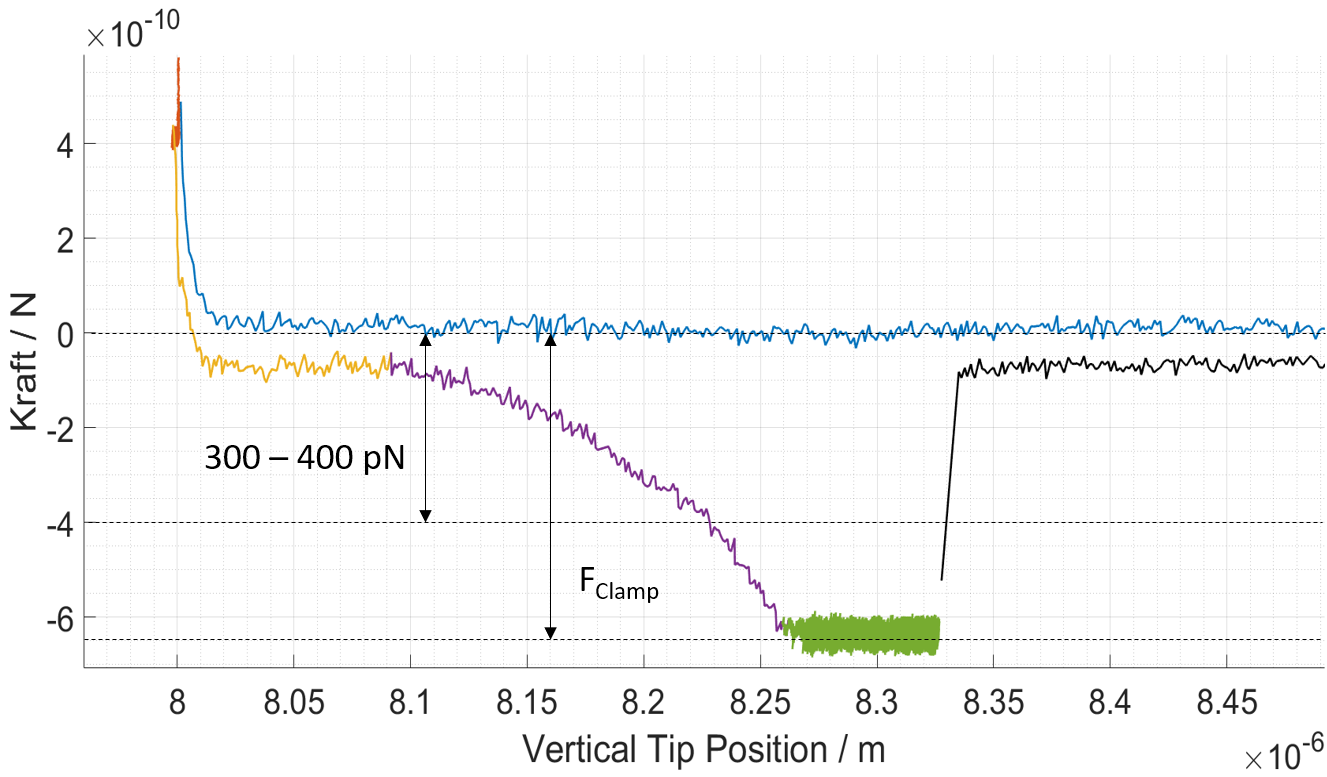
\includegraphics[width=\textwidth]{Abbildungen/Bsp_Force_Clamp_F_vs_x_IV.png}
		} % scalebox
		\subcaption{}
		\label{subfig:kraft_abstand}		
	\end{subfigure}
	\begin{subfigure}[b]{\textwidth}
		\centering
		\scalebox{\hscaleZero}{
			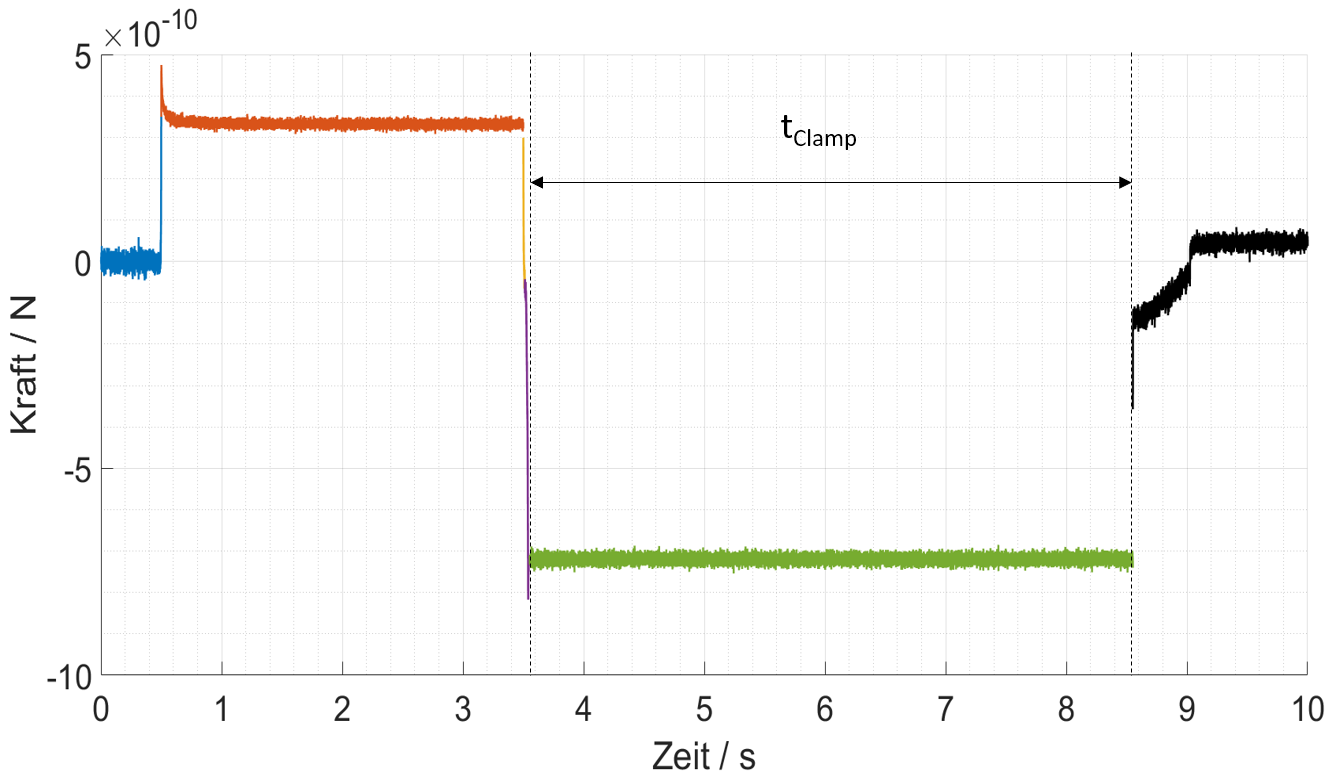
\includegraphics[width=\textwidth]{Abbildungen/Bsp_Force_Clamp_F_vs_t_III.png}
		} % scalebox
		\subcaption{}
		\label{subfig:kraft_zeit}			
	\end{subfigure}
	\caption[Beispiele einer Force-Clamp-Kraftkurve]{Beispiele einer Force-Clamp-Kraftkurve: a) Kraft-Abstand-Kurve. Hervorgehoben ist das \acs*{CMA}-spezifische Plateau bei 300 - 400 pN. b) Kraft-Zeit-Kurve. Hervorgehoben ist die Clampzeit dieser Kraftkurve von $t_{Clamp}~=~5,02~s$. Blau: Hinfahrkurve. Orange: Ruhezeit. Gelb: Initial Retract. Lila: Clamp Retract. Grün: Retract. Schwarz: Retract.}
	\label{fig:force_clamp_kurve}
\end{figure}

\subsection{Auflösungsgrenzen der Kraftexperimente}
\label{subsec:auflösungsgrenzen_der_kraftexperimente}

Über die \samplerate~wird bestimmt, mit welcher Datenauflösung Force-Clamp-Experimente in den einzelnen Domänen (Zeit, Weg und Kraft) aufgenommen werden können. Datenauflösung bedeutet in diesem Zusammenhang, wie klein ein bestimmtes Intervall (Zeitintervall, Wegintervall oder Kraftintervall) sein darf, sodass eine Mindestanzahl von Datenpunkten nicht unterschritten wird. Die \samplerate~ist folgendermaßen definiert:

\begin{equation}
	f_r = \frac{Datenpunkte}{Zeitintervall} = \frac{c}{\Delta t}
\end{equation}

Für die \samplerate~gilt:

\[ \frac{c}{\Delta t} = \frac{c_{min}}{\Delta t_{min}} \]

Damit folgt für das kleinste Zeitintervall:

\begin{equation}
	\Delta t_{min} = c_{min} \cdot \frac{\Delta t}{c} =  \frac{c_{min}}{f_r}
\end{equation}

Für mindestens einen Datenpunkt in $\Delta t_{min}$, muss $c_{min} = 1$ gelten:

\begin{equation}
		\Delta t_{min} = \frac{1}{f_r}
\end{equation}

$\Delta t_{min}$ kann über die Zuggeschwindigkeit $v$ in das minimale Wegintervall $\Delta l_{min}$ umgerechnet werden:

\begin{equation}
	\Delta l_{min} = v \cdot \Delta t_{min} = v \cdot \frac{c_{min}}{f_r}
\end{equation}

Für $\Delta l_{min}$ gilt ebenfalls $c_{min} = 1$:

\begin{equation}
	\Delta l_{min} = \frac{v}{f_r}
\end{equation}

 $\Delta l_{min}$ kann wiederum über die Federkonstante des Cantilevers $k_{Spring}$, in das minimale Kraftintervall $\Delta F_{min}$ umgerechnet werden:

\begin{equation}
	\Delta F_{min} = k_{Spring} \cdot \Delta l_{min} = k_{Sping} \cdot v \cdot \Delta t_{min} = \frac{k_{Spring} \cdot v}{f_r} \cdot c_{min}
\end{equation}

Für $\Delta F_{min}$ muss ebenfalls $c_{min} = 1$ gelten:

\begin{equation}
	\Delta F_{min} = \frac{k_{Spring} \cdot v}{f_r}
\end{equation}

Typische Werte für $f_r$, $v$\footnote{$v$ bezieht sich auf das 5. Segment (Clamp-Retract) eines Force-Clamp-Experiments. In diesem Segment wurde die \amid~bis auf die vorgesehene Kraft ($800~pN$) gestreckt.} und $k$ sind:

\begin{itemize}
	\item $f_r = 5000~s^{-1}$
	\item $v~= 5~µms^{-1}$
	\item $k_{Spring} = 0,08~Nm^{-1}$
\end{itemize}

Daraus ergeben sich für die jeweiligen Auflösungsgrenzen die folgenden Werte:

\begin{itemize}
	\item $\Delta t_{min} = \frac{1}{f_r} = \frac{1}{5000~s^{-1}} = 0,2 ms$
	\item $\Delta l_{min} = \frac{v}{f_r} = \frac{5 \cdot 10^{-6}~ms^{-1}}{5000~s^{-1}} = 1 \cdot 10^{-9}~m = 1~nm$
	\item $\Delta F_{min} = \frac{k_{Spring} \cdot v}{f_r} = \frac{0,08~Nm^{-1} \cdot 5 \cdot 10^{-6}~ms^{-1}}{5000~s^{-1}} = 8 \cdot 10^{-11}~N = 80~pN$
\end{itemize}